\documentclass[tikz,border=2pt]{standalone}
\usepackage{amsmath}
\usepackage{pgfplots}
\pgfplotsset{compat=1.18}
\usetikzlibrary{arrows.meta}
\begin{document}
% Pooling on m = 0 in the two-type signalling game: mu(0) = 0.4 < 1/2, the receiver rejects, both types
% get 0. Deviating to m = 1 pays 0 (rejected, mu' < 1/2) or 2 (accepted, mu' > 1/2) minus the cost:
% type H gets -1 or 1 (c_H = 1), type L gets -3 or -1 (c_L = 3), where mu' = mu(1) is the off-path
% belief. H does not deviate iff the receiver rejects m = 1; L never deviates. Pooling is a PBE for
% mu' in [0, 1/2] (rejection at the tie mu' = 1/2).
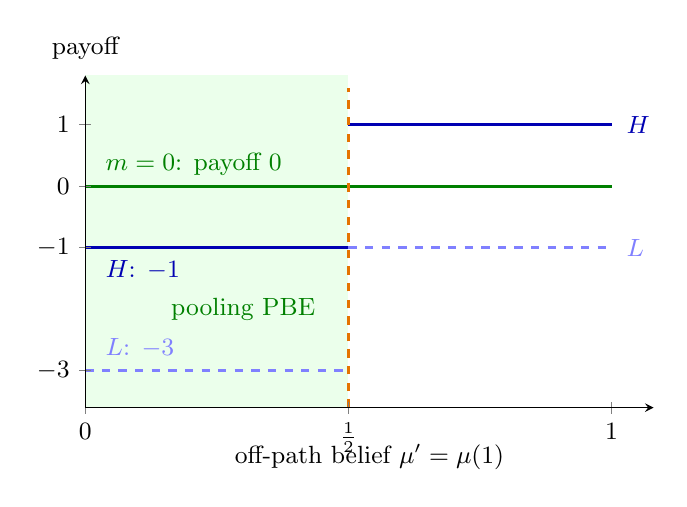
\begin{tikzpicture}[font=\small, >={Latex[length=2mm]}]
  \begin{axis}[
    axis lines=left, xmin=0, xmax=1.08, ymin=-3.6, ymax=1.8,
    xtick={0,0.5,1}, xticklabels={$0$,$\tfrac{1}{2}$,$1$}, ytick={-3,-1,0,1},
    xlabel={off-path belief $\mu'=\mu(1)$},
    ylabel={payoff},
    xlabel style={anchor=north, at={(axis description cs:0.5,-0.08)}},
    ylabel style={rotate=-90, anchor=south, at={(axis description cs:0,1.02)}},
    width=8.8cm, height=5.8cm, clip=false, axis on top]
    % beliefs that support pooling
    \fill[green!8] (axis cs:0,-3.6) rectangle (axis cs:0.5,1.8);
    % pooling payoff
    \addplot[green!50!black, very thick, domain=0:1, samples=2] {0};
    \node[green!50!black, anchor=south west] at (axis cs:0.02,0.02) {$m=0$: payoff $0$};
    % deviation payoffs: rejected for mu' < 1/2, accepted for mu' > 1/2
    \addplot[blue!70!black, very thick] coordinates {(0,-1) (0.5,-1)};
    \addplot[blue!70!black, very thick] coordinates {(0.5,1) (1,1)};
    \addplot[blue!50, very thick, dashed] coordinates {(0,-3) (0.5,-3)};
    \addplot[blue!50, very thick, dashed] coordinates {(0.5,-1) (1,-1)};
    \node[blue!70!black, anchor=west] at (axis cs:1.01,1) {$H$};
    \node[blue!70!black, anchor=north west] at (axis cs:0.02,-1.05) {$H$: $-1$};
    \node[blue!50, anchor=west] at (axis cs:1.01,-1) {$L$};
    \node[blue!50, anchor=south west] at (axis cs:0.02,-2.95) {$L$: $-3$};
    % threshold
    \draw[orange!90!black, thick, dashed] (axis cs:0.5,-3.6) -- (axis cs:0.5,1.6);
    \node[green!50!black] at (axis cs:0.3,-2.0) {pooling PBE};
  \end{axis}
\end{tikzpicture}
\end{document}
